%%%%%%%%%%%%%%%%%%%%%%%%%%%%%%%%%%%%%%%%%%%%%%%%%%%%%%%%%%%%%%%%%%%%%%%%%%%%%
\chapter{Konzept}
\label{chap:concept}
%%%%%%%%%%%%%%%%%%%%%%%%%%%%%%%%%%%%%%%%%%%%%%%%%%%%%%%%%%%%%%%%%%%%%%%%%%%%%
\chapterstart
Um die beschriebenen Problemstellungen zu lösen und diese Ergebnisse auch evaluieren zu können, wird eine Applikation entwickelt. In dieser Applikation werden die Ergebnisse der Statischen Code Analyse aufbereitet, visualisiert und angezeigt. Die Daten müssen für die Möglichkeit einer langfristigen Auswertung dauerhaft in einer Datenbank gespeichert werden. \\\\ Für die Testdaten werden gezielt Tools in verschiedenen Projekten eingesetzt. Die Daten werden in die Datenbank importiert. 
\begin{figure}[tp]
  \centering
  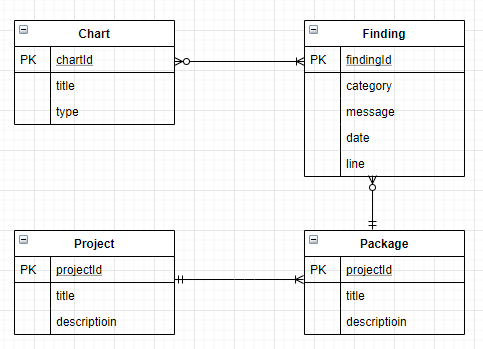
\includegraphics[height=6cm]{images/chartERD.PNG}
  % The short caption should be capitalised
  % The full caption should hold a full sentence. 
 \caption[Beispiel-ERD, mit der die Daten für die weitere Aufbereitung gespeichert werden können.]{Beispiel-ERD, mit der die Daten für die weitere Aufbereitung gespeichert werden können.}
  \label{fig:chartERD}
\end{figure}
Um die Daten in die Datenbank importieren zu können, ist eine zusätzliche Lösung erforderlich. Diese zusätzlich Lösung als Batch-Job, manueller Importer oder als Plugin erstellt werden. Da ein Batch-Job oder ein Importer eine zusätzliches Applikation erfordert, wird in Plugin implementiert. Dieses Plugin kann auch konfiguriert werden, damit der Entwickler oder die Entwicklerin die Datenquellen und den Zeitpunkt des Imports selber festlegen können. In der Abbildung \ref{fig:chartERD} wird eine Möglichkeit dargestellt, wie diese Daten in der Datenbank gespeichert werden können und so als Basis für die Visualisierungen und Tabellen dienen können. \\\\
In der der Applikation können die Benutzer und Benutzerinnen die Daten gezielt auslesen. Da die Daten eine große Menge an Daten über einen großen Zeitraum gespeichert werden sollen, ist eine Filterung der Daten notwendig. Die Visualisierungen in der Applikation betreffen die Fehler und versuchen Fragen zu lösen wie: Wo sind die meisten Fehler aufgetreten? Was sind die häufigsten Fehler und wie kann man die Fehler vermeiden? Welche packages erfordern ein Refactoring? Diese Fragen sollen in Charts beantwortet werden, die mit den Daten automatische generiert werden. Die Applikation ist daher für den einzelnen Entwickler, als auch für das ganze Entwicklungs-Team von Interesse. Diese Informationen sollen auch als Information versendet oder gespeichert werden können, daher soll ein Export der Daten möglich sein. Der Export wir als PDF-Dokument generiert, da so alle Daten formatiert und gelistet ausgegeben werden können. \\\\ Die Applikation wird als Webapplikation entwickelt. Dies bietet den Vorteil, dass die Daten und mögliche Einstellungen und Konfigurationen für alle Entwicklerinnen und Entwickler verfügbar sind und die Webapplikation zentral für alle verfügbar ist. Ein Nachteil, gegenüber einer Desktopapplikation oder einer Extension für die Entwicklungsumgebung ist hierbei die fehlende Möglichkeit, direkt und automatisch zu den Fehlerquellen zu navigieren. Der Fokus der Webapplikation richtet sich aber auf die Übersicht, Visualisierung und die kontinuierliche Verbesserung des Codes der Benutzerinnen und Benutzer. \\\\ Die Visualisierungen sollen so erstellt werden, das sie unabhängig der eingesetzten Tools erstellt werden können. Die Visualisierungen sollen modern und einfach verständlich präsentiert werden.


%Your text here\ldots
%Describe an overall concept of a solution, which could possibly solve a given problem. Design a novel solution and visualise the architecture and relevant (data) flows. Compare and relate your approach to possible alternatives and argue why the suggested solution will be better. woher testdaten; wie vorgehn bei entwicklung; was soll gelöst werden; was soll noch kommen;

\chapterend